\section{Implementation}\label{impl}
This section overviews the implementation of SCache -- a distributed in-memory storage system that caches shuffle data of DAG framework. Here we use Spark as example of DAG framwork to illustrate working process of shuffle optimization. We will first present system architecture in Subsection \ref{arch} while the following two subsections focuss on the two main challenges: memory manangement and fault tolerence.

\subsection{System Architecture}\label{arch}
SCache consists mainly two components: A distributed in-memory shuffle data storage system and the daemon inside Spark. As shown in Figure \ref{fig:arch}, for the in-memory storage system, SCache employs the legacy master-slaves architecture like GFS\cite{gfs}. The master node of SCache coordinates the shuffle blocks globally with application context from Spark. The coordination provides two guarantees: (a)store data in memory before tasks start and (b)schedule data on-off memory with all-or-nothing property and strict priority constraints to benifit all jobs. 

When a Spark job starts, the DAG will be first generated by Spark DAGScheduler\cite{sparksource}. The process starts on the last result stage, and recursively find the dependent stages until the beginning of the DAG. While going forward to the beginning, the DAG computing pipeline will be cut off if a RDD in the stage has one or more shuffle dependencies. These shuffle dependencies among RDDs will then be submitted through RPC call to SCache master by a daemon process in Spark driver. For each shuffle dependency, the shuffle ID(an integer generated by Spark), the type of partitioner, the number of map tasks and the number of reduce tasks are included in the RPC call. The SCache master will store the metadata of one RPC call as a set of mutilpule shuffles scheduling unit. If there is a specialized partitioner, such as Range Partitioner or a customed paritioner, in the shuffle dependencies, the daemon will insert a sampling program in the host RDD that generates shuffle output using specialized partitioner. The sampling application will be scheduled ahead of that host RDD. We will illustrate the sampling procedure in the Section \ref{sampling}.

For the hash partitioner, when the map tasks in a stage finish computing on the work nodes, the  SCache Worker Daemon process will hijack the shuffle map output in the JVM of each executor of Spark (see Figure \ref{fig:arch}). Then the data will be transfered into the reserved memory of SCache Worker on each node through memory copy. In the same time, the Spark tasks will end after the memory copy without the disk shuffle output writing, which leads to a  reduction of the whole tasks completion time. When the shuffle map output block of a task is stored in the reserved memory, the SCache worker will then notify the master of the block belonging information with the reduce size distribution in this block (see Map Output in Figure \ref{fig:shuffle}). When the collected map output data reach the observed raito of map output, the SCache master will then run the scheduling algorithm \ref{mhminheap} (for multiple shuffle dependencies) and \ref{hminheap} (for single shuffle dependency) to get the reduce tasks -- nodes mapping. When the scheduling resulted is made, the master will then notify each worker to prepare the memory space for the shuffle data for reduce tasks. The pre-fetch of shuffle data as soon as each worker receives the scheduling results. More specifically, each worker will check the ID of reduce tasks that will be scheduled on itself in the future. When a map task finishs, each node will receive a broadcast message. It will then trigger the pre-fetch process to start fetching shuffle data from the memory of remote SCache worker that just finishs the map task. After all blocks of shuffle map output is transferred, the SCache worker will flush these blocks to disks for saving memory space and fault tolerence. 

Before the reduce stage starts, Spark DAG Scheduler will first generate a task set for this stage with different locality levels -- \textbf{\textit{PROCESS\_LOCAL, NODE\_LOCAL, NO\_PREF, RACK\_LOCAL, ANY}}. The locality levels are set by finding a cached location of a RDD. For the RDDs that have narrow dependency(oppsite ot shuffle dependency), the prefered location can also be the same as the depedent RDDs. For those RDDs that have shuffle dependecies, the locality will be set as \textbf{\textit{NO\_PREF}} by default. To enforce SCache pre-allocated the reduce tasks, we insert some lines of codes in Spark DAG Scheduler to consult SCache Master to get the preferred node for each tasks. By doing this, the tasks with shuffle dependencies can be set as \textbf{\textit{NODE\_LOCAL}}. Then the Task Scheduler will schedule tasks according to the task -- node mapping from SCache. 

When the scheduled reduce tasks start, the shuffle input data is requested. The SCache worker will then pass the requested data through memory copy from the reserved memory to Spark executor JVM memory. 

\subsubsection{Reservior Sampling}\label{sampling}
If the submitted shuffle dependencies contain a Rrange Partitioner or a customed partitioner, the SCache master will send a sampling request to the daemon process in Spark driver. The daemon process will then submit a job on Spark for the current RDD. This sampling job will use a reservoir sampling algorithm\cite{reservoir} on each partition of RDD since the items size of each partition is unknow before sampling. For the sample number, we set the size equals to $3 \times number\ of\ partitions$ for balancing overhead and accurancy (it can be tuned by configuration). The sampling job will then perform a local shuffle with the selected items and partitioner (see Figure \ref{fig:sample}). At the same time, the size of items is counted as the weight of each partition.These sampling data will be aggregated by $reduce\ ID$on SCache master. The size for each reduce partition can be easily computed by equation \ref{equationsample}. After the prediction, master will call algorithm \ref{mhminheap} and \ref{hminheap} to do the scheduling. 

\subsection{Memory Management}
As mentioned in section \ref{shufflesize}, the shuffle size is small enough that can be easily fit in memory. In order to minimize the reserved memory of SCache worker on each node, the probablity of memory exceeded is still exist, especially for multipule existing applicaitons scenrios. To achieve maximum imporvment in overall, SCache leverages two constraints to manage the in-memory data -- all-or-nothing and  strict priority property.
\subsubsection{All-or-Nothing Property}
Achieving memory cached shuffle data for a reduce task will shorten the task execution time. But this acceleration of single task doesn't speed up the whole stage. For a stage that contains multiple tasks, the completion time depends on the timestamp of last task. Therefore, the memory cache of shuffle data need to match every task in a stage. We refer to this as the all-or-noting property. 
\subsubsection{Strict priority}
When the size of cached shuffle data exceeds the reserved memory, SCache will decide which of these should be flushed to disk according to the priorities of each data blocks. 


\begin{figure}
	\centering
	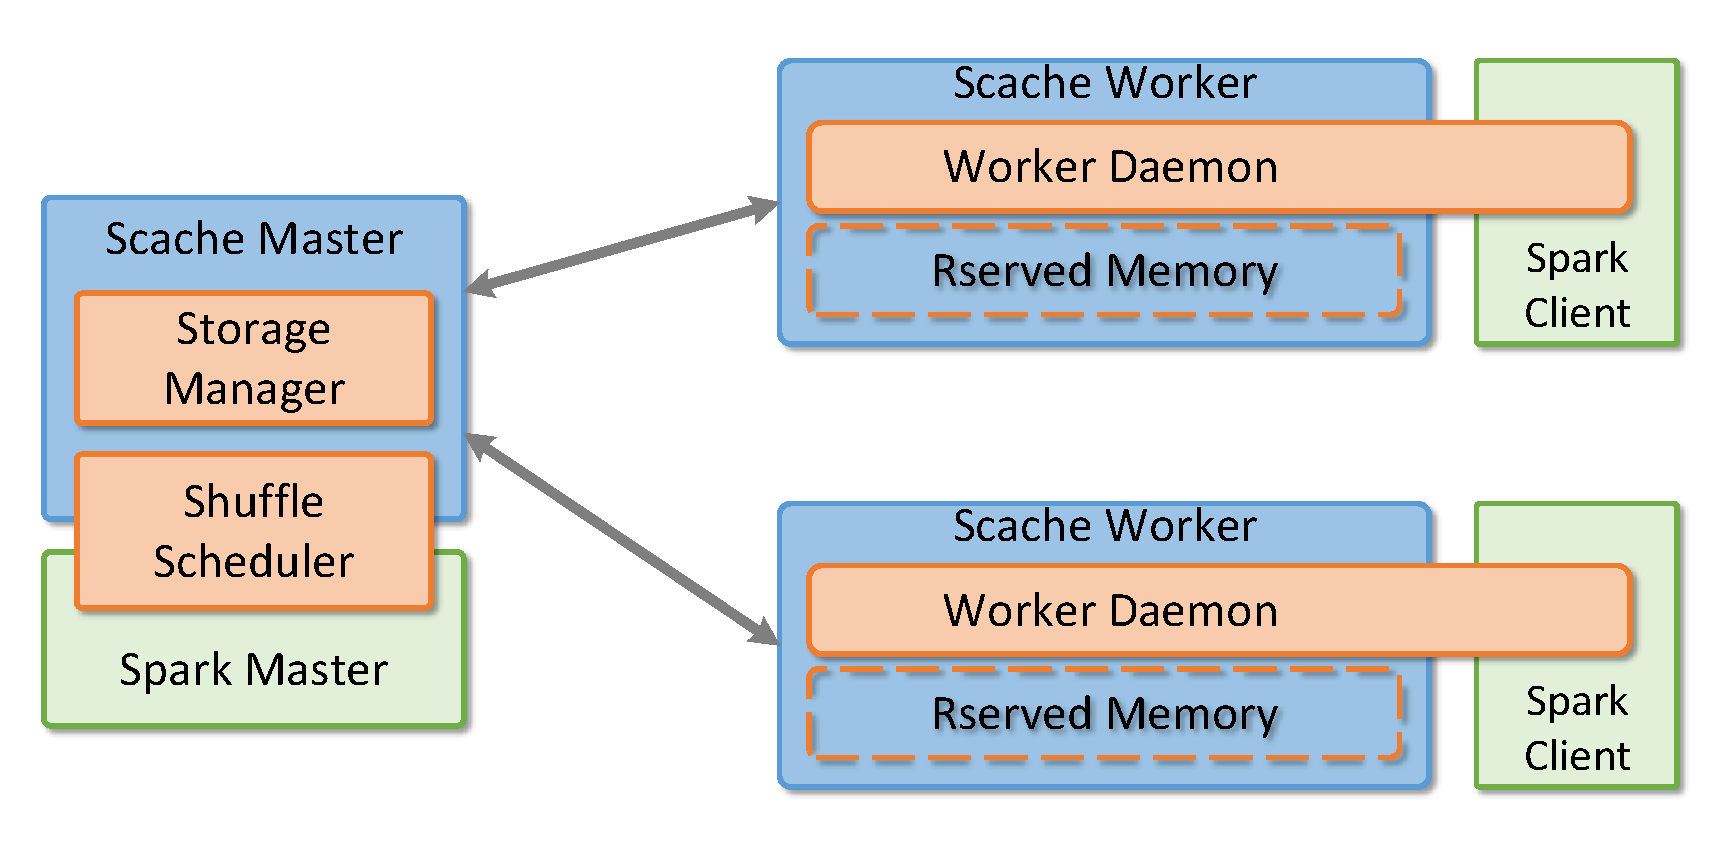
\includegraphics[width=\linewidth]{fig/arch}
	\caption{SCache Architecture}
	\label{fig:arch}
\end{figure}
\begin{figure}
	\centering
	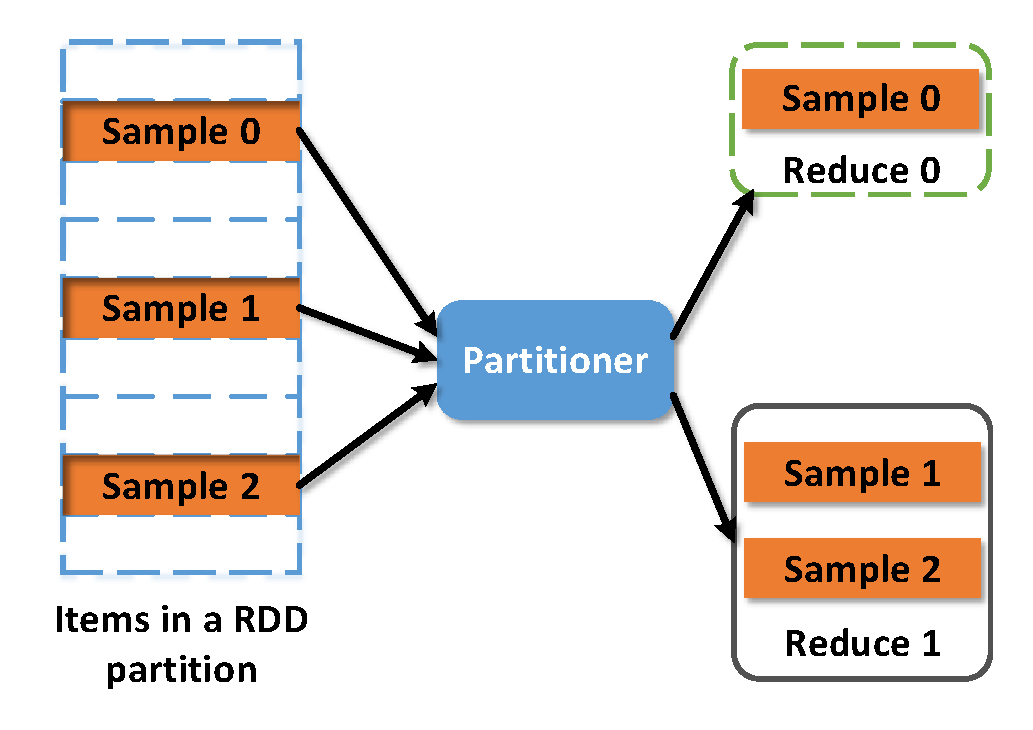
\includegraphics[width=\linewidth]{fig/sample}
	\caption{Demonstration of Reservoir Sampling}
	\label{fig:sample}
\end{figure}